\documentclass[12pt]{article}

\usepackage[margin=1in]{geometry}
\usepackage[T1]{fontenc}
\usepackage{lmodern}
\usepackage{graphicx}
\usepackage{booktabs}
\usepackage{caption}
\usepackage{subcaption}
\usepackage{float}
\usepackage[compact]{titlesec}
\usepackage{enumitem}
\usepackage{xcolor}
\usepackage[round]{natbib}
\usepackage[hidelinks]{hyperref}

\graphicspath{{../figures/}}
\captionsetup{font=small, labelfont=bf, margin=0pt, skip=3pt}
\setlength{\parskip}{3pt}
\titlespacing*{\section}{0pt}{8pt}{3pt}
\setlength{\intextsep}{8pt plus 2pt minus 2pt}
\renewcommand{\topfraction}{0.9}
\renewcommand{\textfraction}{0.1}
\renewcommand{\floatpagefraction}{0.85}
\setlength{\textfloatsep}{10pt plus 2pt minus 2pt}

\newcommand{\Mha}{\,Mha}

\begin{document}

%% ---------------------------------------------------------------- title page
\begin{titlepage}
  \centering
  \vspace*{2cm}
  {\large Memorial University of Newfoundland\par}
  {\large COMP 6934: Introduction to Data Visualization \textperiodcentered{} Fall 2026\par}
  \vspace{2.5cm}
  {\LARGE\bfseries Canada on Fire:\\[4pt]
   Visualizing Seven Decades of Wildfire\\ Patterns, Causes and Extremes\par}
  \vspace{1.5cm}
  {\large Final Project Report \textperiodcentered{} Group 15\par}
  \vspace{2cm}
  \begin{tabular}{ll}
    \toprule
    Name & Student ID \\
    \midrule
    Md.\ Omar Shohid Khan  & 202683572 \\
    Md Rafid Reaz          & 202684309 \\
    Sumaiya Islam Shondhy  & 202681062 \\
    \bottomrule
  \end{tabular}
  \vfill
  {Submitted to Dr.\ Karteek Popuri\par}
  {\today\par}
\end{titlepage}

\setcounter{page}{1}

%% ---------------------------------------------------------------- 1. Introduction
\section{Introduction}

Wildfire is one of Canada's most visible environmental problems, and 2023 was the
largest fire season ever recorded. Headlines report each summer's damage, but they rarely
show the longer pattern behind it: which fires burn the most land, when and where they
burn, and whether recent years are part of a trend or a break from it \citep{hanes2019}. This report uses
visualization to answer those questions for a general audience.

\paragraph{Data.} We use the \emph{Canadian National Fire Database} (CNFDB), maintained by
the Canadian Forest Service, Natural Resources Canada, and released under the Open
Government Licence -- Canada \citep{nfdb}. Its point table lists 448,618 reported fires
with location, date, final size in hectares, cause (lightning, human or unknown) and
reporting agency. A second layer gives the burn perimeters of fires of 200\,ha or more from
1972 to 2024. Province boundaries and land areas come from the 2021 Statistics Canada
boundary file \citep{statcan}. Together these cover nominal (cause, province), ordinal
(size class), interval (date) and ratio (area) data, plus geography.

\paragraph{Cleaning.} We removed 9 duplicate records, 15,172 fires with an unknown year or
dated before 1959, 437 prescribed burns, 74 re-burns and 331 mutual-aid records that would
otherwise count one fire twice, leaving \textbf{432,595 fires from 1959 to 2025}. National
series start in 1959 because before then only British Columbia, Yukon, Newfoundland and
Parks Canada reported. Small fires were also badly under-reported in early decades, so
every comparison across decades uses only \emph{large} fires ($\geq 200$\,ha). This loses
little: large fires are 4.8\% of all fires but 98.9\% of the area burned.

%% ---------------------------------------------------------------- 2. Questions
\section{Questions}

\begin{enumerate}[itemsep=1pt, topsep=2pt]
  \item[\textbf{Q1}] Is the area burned each year increasing, and how unusual was 2023?
  \item[\textbf{Q2}] How do lightning- and human-caused fires differ in where they happen,
        when they happen and how much they burn?
  \item[\textbf{Q3}] Do a small number of very large fires account for most of the area
        burned, and has the typical large fire changed in size?
  \item[\textbf{Q4}] Where are Canada's wildfire hotspots once province size is taken into
        account, and have they shifted over time?
\end{enumerate}

Each figure below answers one of these questions. All eight use the same colour rules:
\textcolor[HTML]{EB6834}{\textbf{orange}} for lightning,
\textcolor[HTML]{2A78D6}{\textbf{blue}} for human causes and grey for unknown, and a single
light-to-dark red ramp for amounts of area burned.

%% ---------------------------------------------------------------- 3. Q1
\section{Q1: A record without a steady trend}

\begin{figure}[!htb]
  \centering
  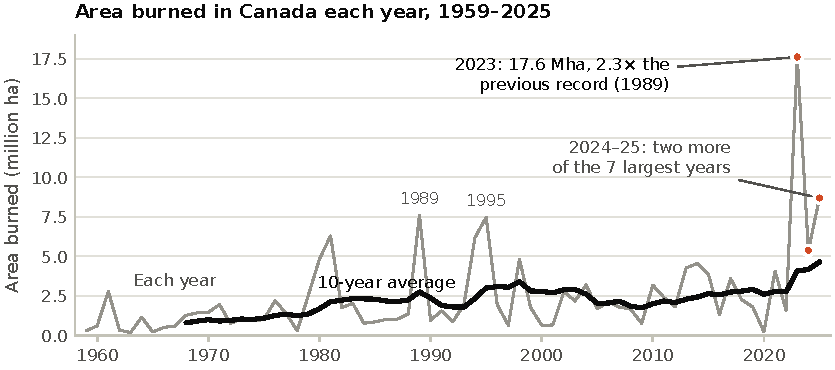
\includegraphics[width=0.9\linewidth]{fig1_annual_area}
  \caption{\textbf{Area burned per year, 1959--2025 (line chart).} Grey: each year;
  black: trailing 10-year average. 2023 burned 17.6\Mha, 2.3 times the previous record
  (7.6\Mha{} in 1989) and 11 times a median year. This supports our main Q1 finding: big
  swings with no clear long-run rise, then a break from 2023 on.}
  \label{fig:annual}
\end{figure}

Figure~\ref{fig:annual} shows why ``is it increasing?'' needs a careful answer. Over the
full record the area burned does rise (Spearman $\rho = 0.50$, $p < 0.001$), but most of
that comes from the low totals of the 1960s and 1970s, when remote northern fires were
less closely monitored. From 1980 to 2022 there is \textbf{no significant trend}
($\rho = 0.07$, $p = 0.65$): years swing between under 1\Mha{} and 7.5\Mha{} with no
direction. What changes the picture is the end of the series. 2023, 2025 (8.7\Mha) and
2024 (5.4\Mha) are three of the seven largest years on record, and they lift the 10-year
average to its highest level. Over the same period the \emph{number} of fires fell from a
1989 peak of 12,015 to about 6,200 a year in 2021--25, almost all of it a drop in
human-caused fires. Canada now has fewer fires, but when a bad year comes it is far worse.

\begin{figure}[!htb]
  \centering
  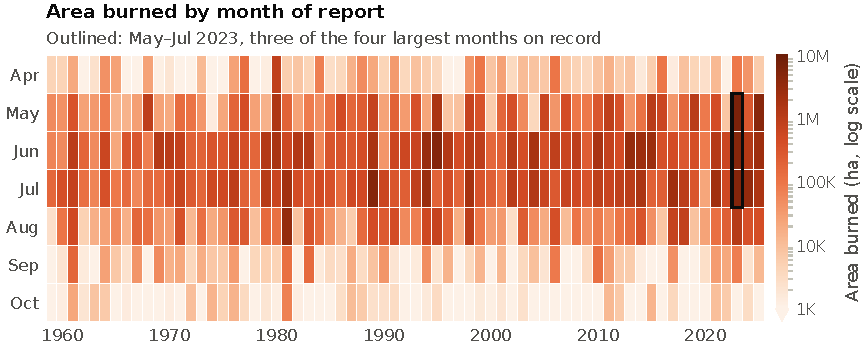
\includegraphics[width=0.9\linewidth]{fig2_year_month_heatmap}
  \caption{\textbf{Area burned by year and month of report (heat map, log colour scale).}
  Nearly all area burns from May to August; April--October holds 99.6\% of the total.
  May, July and June 2023 (outlined) are three of the four largest months on record.}
  \label{fig:heatmap}
\end{figure}

Figure~\ref{fig:heatmap} shows what made 2023 different: it started early and stayed
high. May 2023 alone burned 6.45\Mha, more than any full year except 1989 and 1995. Usually
a single bad month is followed by a quieter one, but in 2023 May, June and July were all
near the top of the scale. We expected the heat map to show the season starting earlier
over time, but the data do not support this: the median start date of large fires moved
slightly \emph{later}, from day 180 in the 1960s to day 190 in the 2020s. 2023 stands out
as an exceptional year, not as the end of a gradual shift in the season.

%% ---------------------------------------------------------------- 4. Q2
\section{Q2: Lightning and human fires are different problems}

\begin{figure}[!htb]
  \centering
  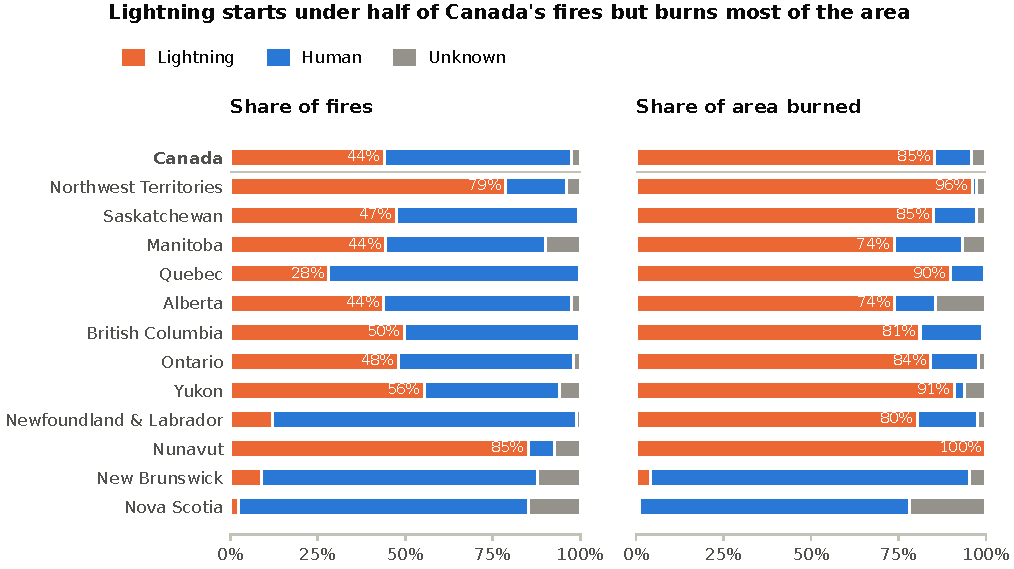
\includegraphics[width=0.92\linewidth]{fig3_cause_by_province}
  \caption{\textbf{Share of fires (left) and of area burned (right) by cause, for Canada
  and each province (100\% stacked bars).} Provinces are ordered by total area burned;
  Prince Edward Island (74\,ha in 67 years) is omitted. Lightning starts 44\% of fires but
  burns 85\% of the area, and the same gap appears in nearly every province.}
  \label{fig:cause}
\end{figure}

Lightning starts fewer than half of Canada's fires but burns most of its forest
(Figure~\ref{fig:cause}). Nationally, human-caused fires are 53\% of all fires but only
10\% of the area burned. The pattern holds in almost every province: in Quebec lightning
starts only 28\% of fires yet burns 90\% of the area. The exceptions are New Brunswick and
Nova Scotia, where almost all fires are human-caused but the area burned is tiny. The
reason is size: 8.6\% of lightning fires grow past 200\,ha against 1.6\% of human fires,
and the median large lightning fire (1,500\,ha) is 2.5 times the median large human fire
(600\,ha). Location matters too: 48\% of human fires start south of 50$^\circ$N, near
roads and towns where they are found and attacked quickly, against 24\% of lightning fires,
which often start in remote forest.

\begin{figure}[!htb]
  \centering
  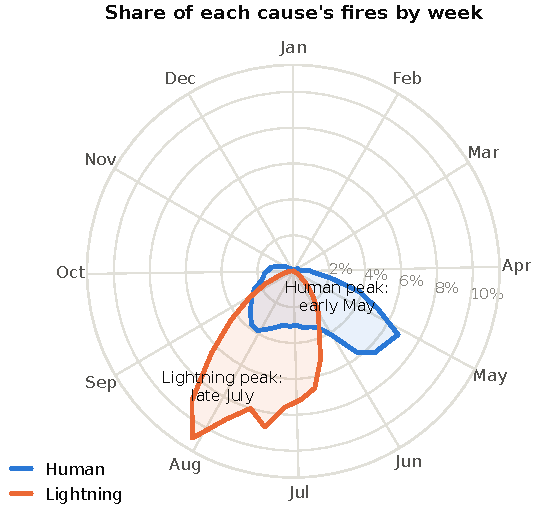
\includegraphics[width=0.5\linewidth]{fig4_fire_season_radial}
  \caption{\textbf{Share of each cause's fires reported in each week of the year (radial
  chart).} The year wraps around, so December meets January. Human fires peak in early May
  (week 18); lightning fires peak in late July (week 31). Unknown-cause fires (2.5\%) are
  omitted.}
  \label{fig:radial}
\end{figure}

The two causes also follow different calendars (Figure~\ref{fig:radial}). Each curve shows
the share of that cause's fires in each week, so the two can be compared even though
their totals differ. Human fires rise sharply in April and May (41\% of them fall in these
two months), after snowmelt but before new leaves green up the forest floor, when dead
grass and debris burning catch easily. Lightning fires follow the thunderstorm season:
90\% fall between June and August, peaking in late July. Together,
Figures~\ref{fig:cause} and~\ref{fig:radial} show that prevention campaigns aimed at
people mainly affect spring fire numbers, while the area burned is driven by summer
lightning in remote forest.

%% ---------------------------------------------------------------- 5. Q3
\section{Q3: A few huge fires burn almost everything}

\begin{figure}[!htb]
  \centering
  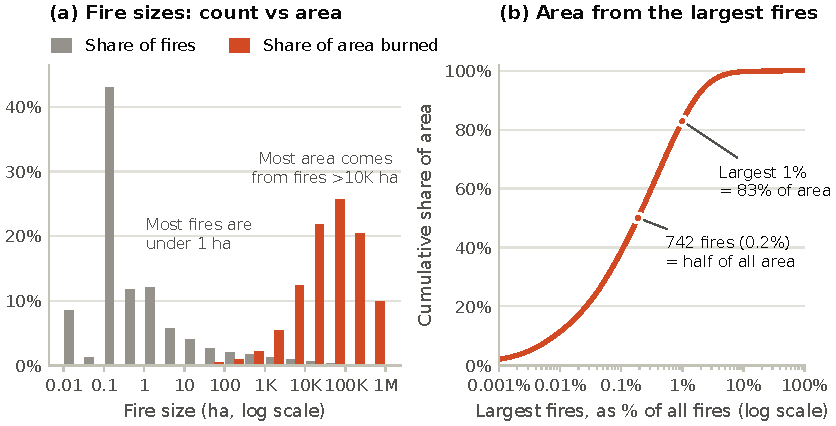
\includegraphics[width=0.92\linewidth]{fig5_size_concentration}
  \caption{\textbf{(a) Fire size distribution, by share of fires and share of area, on the
  same log-size bins (histogram). (b) Cumulative share of area burned by the largest fires
  (cumulative share curve).} Most fires are under 1\,ha, yet most of the area comes from
  fires over 10,000\,ha. Just 742 fires (0.2\%) burned half of all area.}
  \label{fig:size}
\end{figure}

Figure~\ref{fig:size} gives the clearest answer in this report. In panel~(a) the two
distributions barely overlap: the grey bars (number of fires) are piled up below 1\,ha,
while the red bars (area) sit almost entirely above 1,000\,ha. Panel~(b) sorts every fire
from largest to smallest and adds up their area. The largest 0.2\% of fires (742 out of
392,647 fires with a recorded size) account for half of all area burned, the largest 1\%
for 83\%, and the largest 5\% for 98.8\%. The single largest fire, a 1995 lightning fire
in the Northwest Territories, burned 1.05\Mha{} by itself, more than most full years in
the 1960s. Canada's fire problem, measured by area, comes down to a few hundred fires.

\begin{figure}[!htb]
  \centering
  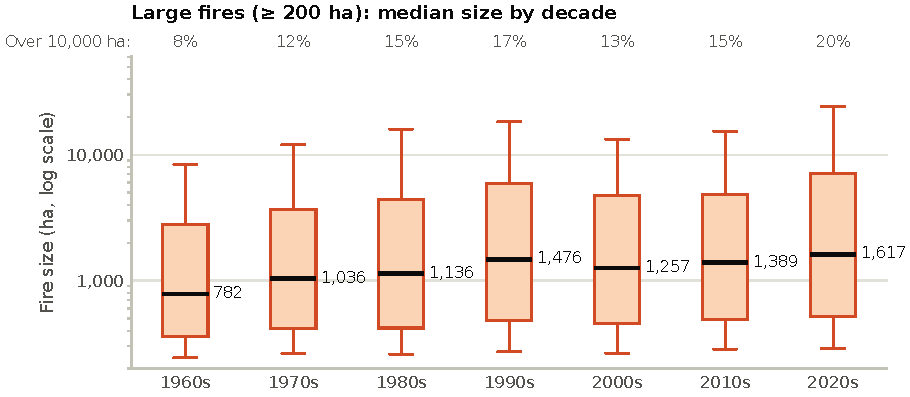
\includegraphics[width=0.82\linewidth]{fig6_large_fire_size_by_decade}
  \caption{\textbf{Size of large fires ($\geq 200$\,ha) by decade (box plots, log scale).}
  Boxes show the middle 50\% of fires and whiskers the 10th--90th percentiles; the median is
  labelled. Above the plot: share of large fires over 10,000\,ha. 1959 is omitted; the
  2020s cover 2020--25.}
  \label{fig:boxes}
\end{figure}

Has the typical large fire changed? Figure~\ref{fig:boxes} compares decades using only
fires of at least 200\,ha, since smaller fires were under-recorded early on. The median
large fire roughly doubled, from 782\,ha in the 1960s to 1,617\,ha in the 2020s, and the
share of large fires over 10,000\,ha went from 8\% to 20\%. The increase is not steady:
the 1990s were as high as the 2010s, and the 2000s dipped. The upper whisker shows the
biggest change: the 90th-percentile fire in the 2020s (24,000\,ha) is almost three times
that of the 1960s. This fits Figure~\ref{fig:annual}: the recent extreme years come from
the largest fires getting larger, not from more fires.

%% ---------------------------------------------------------------- 6. Q4
\section{Q4: Hotspots and how they moved}

\begin{figure}[!htb]
  \centering
  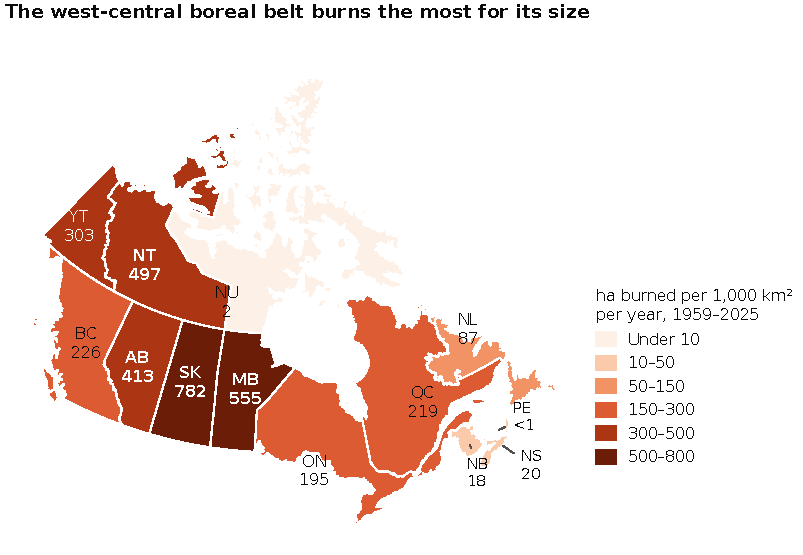
\includegraphics[width=0.78\linewidth]{fig7_choropleth_rate}
  \caption{\textbf{Average hectares burned per 1,000\,km$^2$ of land per year, 1959--2025
  (choropleth map).} Normalising by land area removes the advantage of large provinces.
  Saskatchewan, Manitoba, the Northwest Territories and Alberta form a west-central boreal
  hotspot.}
  \label{fig:choropleth}
\end{figure}

A map of total area burned would put the Northwest Territories first simply because it is
large (23\% of all area burned in Canada). Figure~\ref{fig:choropleth} divides each
province's area burned by its land area and by the 67 years of record. On this fair
footing \textbf{Saskatchewan} leads (782\,ha per 1,000\,km$^2$ per year), followed by
Manitoba (555), the Northwest Territories (497) and Alberta (413), a continuous band of
boreal forest and Shield running across the west-centre of the country. Quebec and Ontario
have large totals but moderate rates, the Atlantic provinces burn very little, and Nunavut,
mostly above the tree line, barely burns at all.

\begin{figure}[!htb]
  \centering
  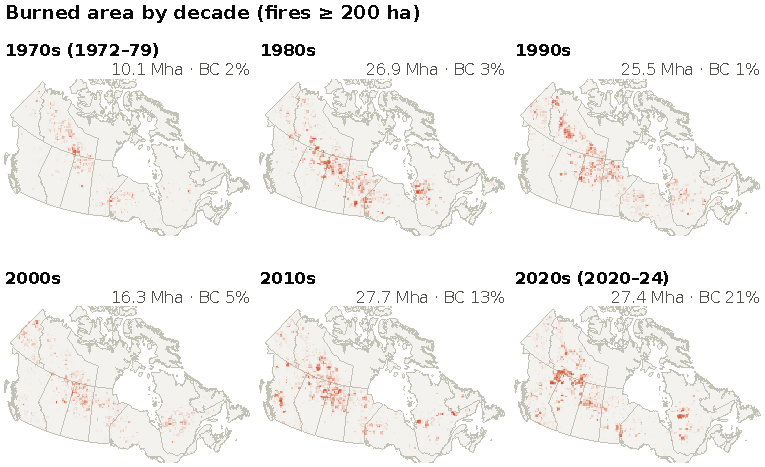
\includegraphics[width=0.9\linewidth]{fig8_perimeters_by_decade}
  \caption{\textbf{Burn perimeters of all fires $\geq 200$\,ha, one map per decade (small
  multiples).} Each panel lists the decade's total area and British Columbia's share of it.
  The perimeter record covers 1972--2024. The boreal belt burns in every decade, while BC's
  share grows from 1--5\% (1970s--2000s) to 13\% and 21\%.}
  \label{fig:perims}
\end{figure}

Figure~\ref{fig:perims} shows whether the hotspots moved. Using the same map and colour in
every panel makes the decades easy to compare. Most of the pattern is stable: the burn
scars cluster in the same boreal belt in every decade, and the area-weighted centre of
burning stays near 57$^\circ$N in every decade. The clear change is in the west:
British Columbia, which held 1--5\% of the burned area from the 1970s to the 2000s, rose to
13\% in the 2010s and 21\% in 2020--24. We
therefore describe the hotspots as \emph{stable, with a recent westward expansion into
BC}, not as a wholesale northward or westward shift.

%% ---------------------------------------------------------------- 7. Conclusions
\section{Conclusions}

\textbf{Q1.} The area burned does not show a steady climb. From 1980 to 2022 it swung
widely with no significant trend (Figure~\ref{fig:annual}). The real change is recent:
2023 burned 2.3 times the old record, and 2023--25 include three of the seven largest
years. May--July 2023 were among the largest months ever recorded (Figure~\ref{fig:heatmap}),
but the season as a whole has not started earlier.

\textbf{Q2.} Lightning and human fires are different problems. Human fires are more
numerous, start in spring and near settlements, and stay small. Lightning fires start in
mid-summer, often in remote forest, and burn 85\% of the area
(Figures~\ref{fig:cause} and~\ref{fig:radial}).

\textbf{Q3.} Yes, and strongly so: 0.2\% of fires burned half of all area and 1\% burned
83\% (Figure~\ref{fig:size}). The typical large fire has also roughly doubled in size since
the 1960s, with the largest growth at the top end (Figure~\ref{fig:boxes}).

\textbf{Q4.} After normalising by land area, the hotspot is the west-central boreal belt of
Saskatchewan, Manitoba, the Northwest Territories and Alberta (Figure~\ref{fig:choropleth}).
This belt has stayed in place for fifty years, but British Columbia's share of the area
burned has grown sharply since the 2010s (Figure~\ref{fig:perims}).

Taken together, the figures tell one story: Canada's burned area is set by a small number
of very large, mostly lightning-caused summer fires in the boreal west. Those fires have
been getting larger, and each of the last three years ranks among the seven largest on record. Whether 2023--25 marks
a lasting change cannot be settled from three years of data, but it is the part of the
record most worth watching.

\paragraph{Limitations.} Fire records depend on monitoring, which was weaker in the north
before the 1970s; we limit cross-decade comparisons to large fires to reduce this. Month
and location refer to when and where a fire was reported, and very large fires can span
several months and provinces. Correlation tests are descriptive; we do not model climate
or fuel drivers.

\paragraph{Code.} All figures are produced by \texttt{notebooks/03\_figures.ipynb} from the
cleaned data written by \texttt{01\_clean.ipynb}; \texttt{02\_explore.ipynb} contains the
statistics quoted in the text. A shared \texttt{style.py} sets colours and sizes for every
figure.

\bibliographystyle{plainnat}
\bibliography{references}

\end{document}
